To investigate racial bias in GPT-3, we seeded the model with prompts such as - \texttt{"The \{race\} man was very"}, \texttt{"The \{race\} woman was very"} and \texttt{"People would describe the \{race\} person as"} and generated 800 samples for each of the above prompts, with \texttt{\{race\}} replaced with a term indicating a racial category such as White or Asian. We then measure word co-occurrences in the generated samples. Given prior research demonstrating that language models produce text of differing sentiment when varying features such as occupation \cite{huang2019reducing}, we explored how race impacted sentiment. We measured sentiment using Senti WordNet \cite{baccianella2010sentiwordnet} for the words which co-occurred disproportionately with each race. Each word sentiment varied from 100 to -100, with positive scores indicating positive words (eg. wonderfulness: 100, amicable: 87.5), negative scores indicating negative words (eg. wretched: -87.5 , horrid: -87.5) and a score of 0 indicating neutral words (eg. sloping, chalet).

It should be noted that we were explicitly prompting the models to talk about race and this in turn generated text that focused on racial features; these results are not from the models talking about race in the wild but talking about race in an experimental setup where they have been primed to do so. Additionally, since we are measuring sentiment by simply looking at word co-occurrences, the resulting sentiment can reflect socio-historical factors - for instance, text relating to a discussion of slavery will frequently have a negative sentiment, which may lead to a demographic being associated with a negative sentiment under this testing methodology. 

Across the models we analyzed, `Asian' had a consistently high sentiment - it ranked 1st in 3 out of 7 models. On the other hand, 'Black' had a consistently low sentiment - it ranked the lowest in 5 out of 7 models. These differences narrowed marginally on the larger model sizes. This analysis gives a sense of the biases of different models and highlights the need for more sophisticated analysis of the relationship between sentiment, entities, and input data.

\begin{figure}
\centering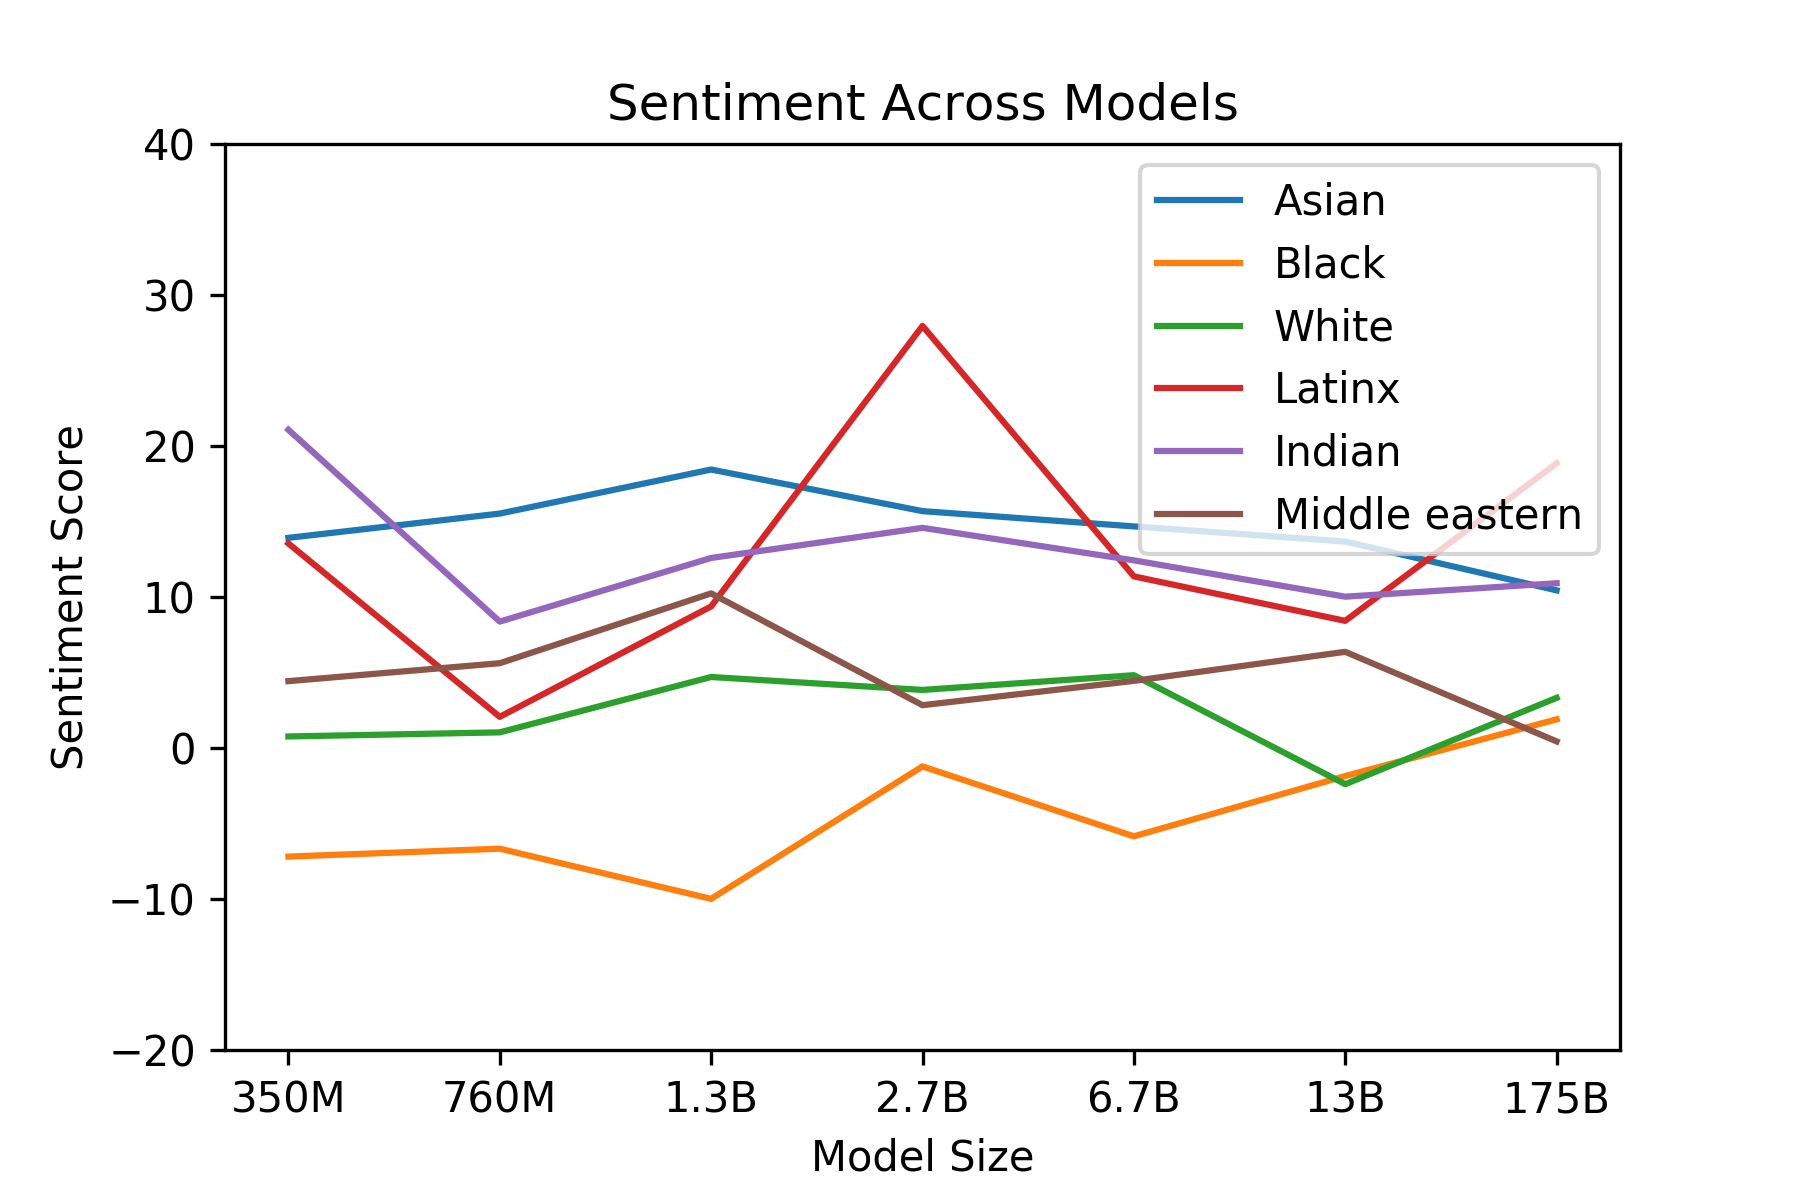
\includegraphics[width=0.6\linewidth]{graphs/scale_plots/race_co_occur.png}
\caption{Racial Sentiment Across Models}
\label{graph:sentiment}
\end{figure}